\documentclass{beamer}
\mode<presentation>
\usepackage{amsmath,amssymb,mathtools}
\usepackage{textcomp}
\usepackage{gensymb}
\usepackage{adjustbox}
\usepackage{subcaption}
\usepackage{enumitem}
\usepackage{multicol}
\usepackage{listings}
\usepackage{url}
\usepackage{graphicx} % <-- needed for images
\def\UrlBreaks{\do\/\do-}

\usetheme{Boadilla}
\usecolortheme{lily}
\setbeamertemplate{footline}{
  \leavevmode%
  \hbox{%
  \begin{beamercolorbox}[wd=\paperwidth,ht=2ex,dp=1ex,right]{author in head/foot}%
    \insertframenumber{} / \inserttotalframenumber\hspace*{2ex}
  \end{beamercolorbox}}%
  \vskip0pt%
}
\setbeamertemplate{navigation symbols}{}

\lstset{
  frame=single,
  breaklines=true,
  columns=fullflexible,
  basicstyle=\ttfamily\tiny   % tiny font so code fits
}

\numberwithin{equation}{section}

% ---- your macros ----
\providecommand{\nCr}[2]{\,^{#1}C_{#2}}
\providecommand{\nPr}[2]{\,^{#1}P_{#2}}
\providecommand{\mbf}{\mathbf}
\providecommand{\pr}[1]{\ensuremath{\Pr\left(#1\right)}}
\providecommand{\qfunc}[1]{\ensuremath{Q\left(#1\right)}}
\providecommand{\sbrak}[1]{\ensuremath{{}\left[#1\right]}}
\providecommand{\lsbrak}[1]{\ensuremath{{}\left[#1\right.}}
\providecommand{\rsbrak}[1]{\ensuremath{\left.#1\right]}}
\providecommand{\brak}[1]{\ensuremath{\left(#1\right)}}
\providecommand{\lbrak}[1]{\ensuremath{\left(#1\right.}}
\providecommand{\rbrak}[1]{\ensuremath{\left.#1\right)}}
\providecommand{\cbrak}[1]{\ensuremath{\left\{#1\right\}}}
\providecommand{\lcbrak}[1]{\ensuremath{\left\{#1\right.}}
\providecommand{\rcbrak}[1]{\ensuremath{\left.#1\right\}}}
\theoremstyle{remark}
\newtheorem{rem}{Remark}
\newcommand{\sgn}{\mathop{\mathrm{sgn}}}
\providecommand{\abs}[1]{\left\vert#1\right\vert}
\providecommand{\res}[1]{\Res\displaylimits_{#1}}
\providecommand{\norm}[1]{\lVert#1\rVert}
\providecommand{\mtx}[1]{\mathbf{#1}}
\providecommand{\mean}[1]{E\left[ #1 \right]}
\providecommand{\fourier}{\overset{\mathcal{F}}{ \rightleftharpoons}}
\providecommand{\system}{\overset{\mathcal{H}}{ \longleftrightarrow}}
\providecommand{\dec}[2]{\ensuremath{\overset{#1}{\underset{#2}{\gtrless}}}}
\newcommand{\myvec}[1]{\ensuremath{\begin{pmatrix}#1\end{pmatrix}}}
\let\vec\mathbf

\title{Matgeo Presentation - Problem 9.2.31}
\author{ee25btech11063 - Vejith}

\begin{document}


\frame{\titlepage}
\begin{frame}{Question}
Find the area of the region bounded by the curve y$^2$=4x and x$^2$=4y
\end{frame}

\begin{frame}{variables}
 \begin{table}[h!]    
  \centering
  \begin{tabular}{|c|c|}
\hline
\textbf{Name} & \textbf{Value} \\ \hline
$\vec{A}$ & $\myvec{2 & 1 \\0 & 3}$ \\ \hline
\end{tabular}

  \caption{Variables Used}
  \label{}
\end{table}   
\end{frame}

\begin{frame}{Solution}
    The equation of a parabola in Matrix form is
\begin{align}
\vec{x}^\top\vec{V}\vec{x} + 2\vec{u}^\top\vec{x} + f = 0
\end{align}
For y$^2$=4x
\begin{align}
    \vec{V_1}=\begin{pmatrix}
        0 & 0\\
        0 & 1
    \end{pmatrix}\\
    \vec{u_1}=-2\vec{e_1}=\myvec{-2\\0}\\
    f_1=0
\end{align}
For x$^2$=4y
\begin{align}
    \vec{V_2}=\begin{pmatrix}
        1 & 0\\
        0 & 0
    \end{pmatrix}\\
    \vec{u_2}=-2\vec{e_2}=\myvec{0\\-2}\\
    f_2=0
\end{align}
\end{frame}

\begin{frame}{Solution}
The intersection of two conics with parameters $\vec{v_i}$,$\vec{u_i}$,f$_i$,i=1,2 is defined as 
\begin{align}
\vec{X}^{T}\,(\vec{V}_{1} + \mu \vec{V}_{2})\vec{X} + 2(\vec{u_1} + \mu \vec{u_2})^{T}\vec{X} \;+\; (f_{1} + \mu f_{2}) \;=\; 0
\end{align}
\begin{align}
\implies \left|
\begin{array}{cc}
\mathbf{V}_1 + \mu \mathbf{V}_2 & \mathbf{u}_1 + \mu \mathbf{u}_2 \\[6pt]
(\mathbf{u}_1 + \mu \mathbf{u}_2)^{\mathrm{T}} & f_1 + \mu f_2
\end{array}
\right| = 0
\end{align}
\begin{align}
    \implies 
\left|
\begin{array}{ccc}
\mu & 0 & -2 \\[6pt]
0 & 1  & -2\mu \\[6pt]
-2 & -2\mu & 0
\end{array}
\right| = 0 \\
\implies \left|
\begin{array}{ccc}
\mu & 0 & -2 \\[6pt]
0 & 1  & -2\mu \\[6pt]
-2 & -2\mu & 0
\end{array}
\right| &\xleftrightarrow{R_3 \leftrightarrow R_3 + \frac{2}{\mu}\times R_1} \left|
\begin{array}{ccc}
\mu & 0 & -2 \\[6pt]
0 & 1  & -2\mu \\[6pt]
0 & -2\mu & -\frac{4}{\mu}
\end{array}
\right|
\end{align}
\end{frame}

\begin{frame}{Solution}
    \begin{align}
&\xleftrightarrow{R_3 \leftrightarrow R_3 + 2\mu \times R_2} \left|
\begin{array}{ccc}
\mu & 0 & -2 \\[6pt]
0 & 1  & -2\mu \\[6pt]
0 & 0 & -(\frac{4}{\mu} +4 \mu ^2)
\end{array}
\right| =0\\
\implies -(4 + +4 \mu ^3)=0\\
\implies \mu=-1
\end{align}
substituting the value of $\mu$=-1 in (8) we get points of intersection as 
\begin{align}
    \vec{x_1}=\myvec{0\\0} \\
    \vec{X_2}=\myvec{4\\4}
\end{align}
\end{frame}
\begin{frame}{Conclusion}
Area of the desired region is given by
\begin{align}
A &= \int_{0}^{4}2\sqrt{x}-\frac{x^2}{4}dx\\
A &= \frac{32}{3}-\frac{16}{3}\\
A &= \frac{16}{3}
\end{align}
\end{frame}

\begin{frame}{Plot}
    \begin{figure}[h!]
    \centering
    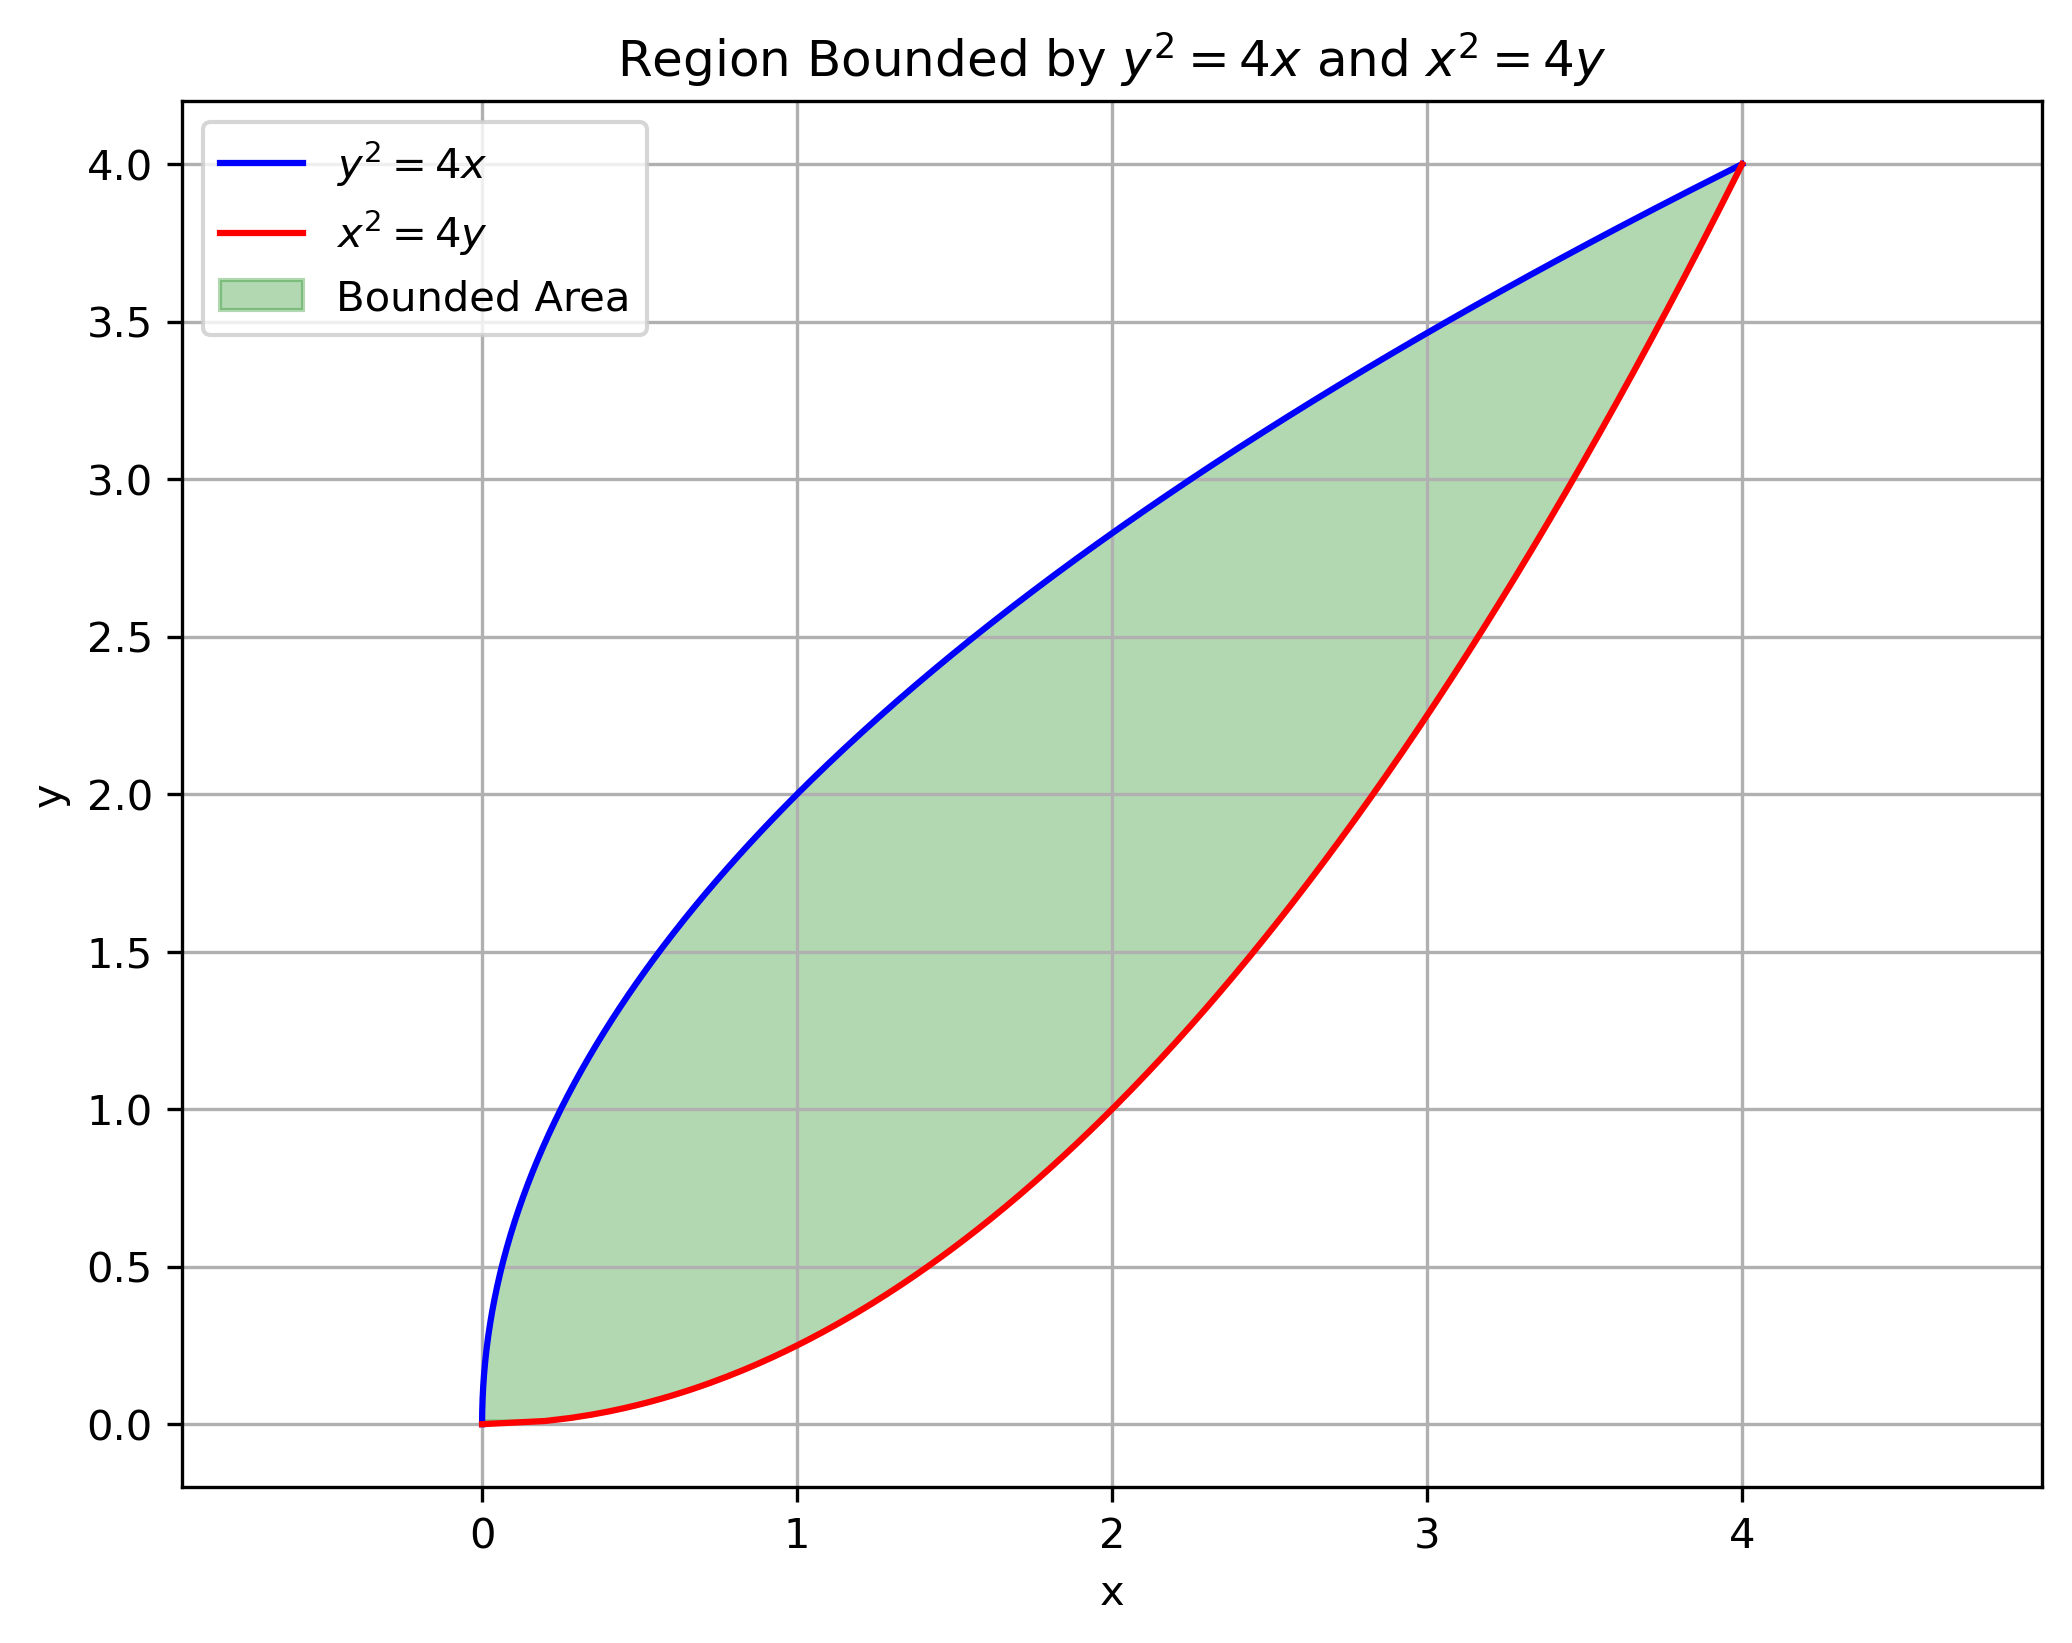
\includegraphics[width=0.7\columnwidth]{figs/01.png}
    \caption{Area bounded}
    \label{fig:placeholder}
\end{figure}
\end{frame}

% --------- CODE APPENDIX ---------
\section*{Appendix: Code}

% C program
\begin{frame}[fragile]{C Code: area.c}
\begin{lstlisting}[language=C]
#include <stdio.h>
#include <math.h>

double f(double y) {
    return 2 * sqrt(y) - (pow(y, 2) / 4.0);
}

int main() {
    double a = 0.0, b = 4.0; // Limits of integration
    int n = 100000; // Number of intervals
    double h = (b - a) / n;
    double area = 0.0;

    for (int i = 1; i < n; i++) {
        double y = a + i * h;
        area += f(y);
    }

    area += (f(a) + f(b)) / 2.0;
    area *= h;

    // Write the result to area.dat
    FILE *fp = fopen("area.dat", "w");
    if (fp == NULL) {
        printf("Error opening file.\n");
        return 1;
    }

    fprintf(fp, "The area bounded by the curves is: %.6lf\n", area);
    fclose(fp);

    return 0;}

\end{lstlisting}
\end{frame}

% Python plotting
\begin{frame}[fragile]{Python: plot.py}
\begin{lstlisting}[language=Python]
import numpy as np
import matplotlib.pyplot as plt

# Define y range (limits from earlier analysis)
y = np.linspace(0, 4, 400)

# Curve 1: y^2 = 4x ⇒ x = y^2 / 4
x1 = y**2 / 4

# Curve 2: x^2 = 4y ⇒ x = 2 * sqrt(y)
x2 = 2 * np.sqrt(y)

# Create the plot
plt.figure(figsize=(8, 6))

# Plot the two curves
plt.plot(x1, y, label=r'$y^2 = 4x$', color='blue')
plt.plot(x2, y, label=r'$x^2 = 4y$', color='red')

# Fill the region between the curves
plt.fill_betweenx(y, x1, x2, where=(x2 > x1), color='green', alpha=0.3, label='Bounded Area')

# Add labels, grid, legend
plt.xlabel("x")
plt.ylabel("y")
plt.title("Region Bounded by $y^2 = 4x$ and $x^2 = 4y$")
plt.legend()
plt.grid(True)
plt.axis('equal')

# Save the figure
plt.savefig("bounded_region.png", dpi=300, bbox_inches='tight')
print("Plot saved as 'bounded_region.png'")

\end{lstlisting}
\end{frame}
\end{document}
